\documentclass[12pt]{beamer}

% Pakete
\usepackage[utf8]{inputenc}
\usepackage[german]{babel}

% AMS Pakete
\usepackage{amsmath}
\usepackage{amsfonts}
\usepackage{amssymb}

% Einheiten
\usepackage{siunitx}
\sisetup{
	output-decimal-marker={,},
	separate-uncertainty
}

% Grafiken
\usepackage{graphicx}


% Theme
\usetheme{Boadilla}
\usecolortheme{rose}
\useoutertheme{infolines}
\useinnertheme{rectangles}
\usefonttheme[onlymath]{serif}

% [num] Zitationen
\setbeamertemplate{bibliography item}[text]

% Navigationsleiste ausschalten
\beamertemplatenavigationsymbolsempty

\DeclareMathOperator{\divergence}{div}

\author[Christopher Deutsch]
{Christopher Deutsch}

\title
{Atomfallen}

\subtitle
{Überblick über die Funktionsweise der wichtigsten Fallen}
%\logo{}

\institute[]
{Rheinische Friedrich-Wilhelms-Universität Bonn \\
Proseminar Präsentationstechnik SS15}

\date{8. Juni 2015}

%\setbeamercovered{transparent}
%\setbeamertemplate{navigation symbols}{}

\begin{document}
\maketitle

\begin{frame}{Inhalt}
	\tableofcontents
\end{frame}


\section{Motivation}

\begin{frame}{Was sind Atomfallen?}
\end{frame}

\begin{frame}{Wofür braucht man Atomfallen?}
	\begin{itemize}
		\item BEC (niedrige Temperaturen)
		\item High-Resolution-Spectroscopy
	\end{itemize}
\end{frame}

\begin{frame}{Grundlagen}
	\begin{itemize}
		\item Fallenpotential und Tiefe
		\item Temperatur der Teilchen (Raumtemperatur $\approx \frac{1}{40} \si{eV}$)
		\item Köhlung?
		
	\end{itemize}
\end{frame}


\section{Ionenfallen}

\begin{frame}{Grundlagen der Ionenfallen}
\end{frame}

\begin{frame}
	1. Maxwell-Gleichung für den ladungsfreien Raum (Quellenfreiheit):
	\begin{align}
	\divergence \vec{E} = 0
	\end{align}
	Gauß'scher Integralsatz:
	\begin{align}
	\int_{V} \divergence \vec{E} \, \mathrm{d}V = \oint_{S = \partial V} \vec{E} \cdot \vec{n} \, \mathrm{d}S = 0
	\end{align}
	Fangen eines positiven Ions in einem Raumvolumen: $\vec{E} \cdot \vec{n} \stackrel{!}{<} 0$
	
	\begin{block}{Earnshaw-Theorem:}
		Ein geladenes Teilchen kann nicht durch elektrostatische Kräfte in einem Raumvolumen gefangen werden.
	\end{block}
\end{frame}

\begin{frame}{Lineare Paul-Falle ($x$-$y$-Ebene)}
	\begin{columns}[t]
		\column{0.5\textwidth}
		Lösung: Verwendung von elektrischen Wechselfeldern
		
		\column{0.5\textwidth}
		\begin{figure}[h]
			\centering
			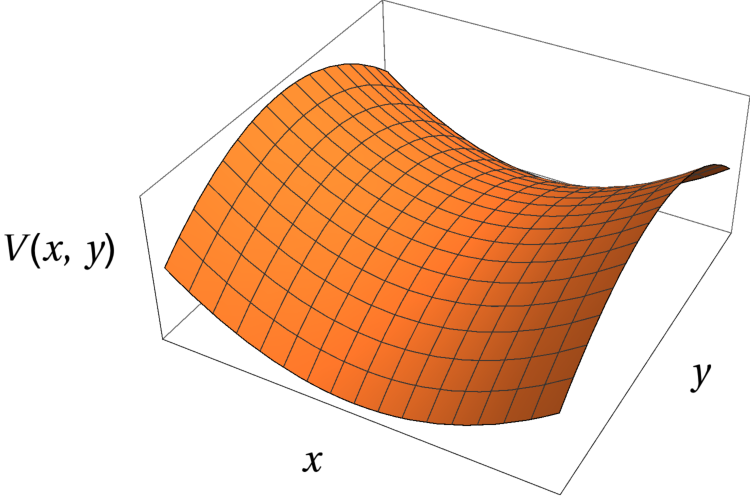
\includegraphics[width=0.95\textwidth]{./figures/sattelpotential.pdf}
			\caption{Sattelpotential}
		\end{figure}
	\end{columns}
\end{frame}

\begin{frame}{Paul-Falle}
\end{frame}

\begin{frame}{Penning-Falle(?)}
\end{frame}


\section{Optische Fallen}

\begin{frame}{Grundlagen: Streukraft}
\end{frame}

\begin{frame}{Grundlagen: Dopplereffekt}
\end{frame}

\begin{frame}{Grundlagen: Feinstruktur und Zeeman-Aufspaltung}
\end{frame}

\begin{frame}{Optische Melasse}
\end{frame}

\begin{frame}{Magneto-optische Falle}
\end{frame}

\begin{frame}{Dipol-Falle (opt. Pinzette) (?)}
\end{frame}


\section{Magnetfalle}

\begin{frame}{Magnetfalle}
\end{frame}


\section{Vergleich}

\begin{frame}{Fallentiefen}
\end{frame}

\section{Literatur}

\begin{frame}{Literatur}
	\begin{thebibliography}{9}
		\bibitem{leo}
		W. R. Leo,
		\emph{Techniques for Nuclear and Particle Physics Experiments},
		Springer 1994
	\end{thebibliography}
	
\end{frame}

\end{document}